
\qrchapter{https://forgottenpillar.com/rsc/en-fp-chapter11}{Umbile la Mungu - na James S. White}

Katika kile kinachofuata, tutachunguza kijitabu cha James White chenye kichwa “\textit{Umbile la Mungu}”. Tunaposoma makala hii, tutaona kwamba James White anaendelea pale ambapo Ndugu Loughborough aliachia, na kwamba anapanua na kuongeza uelewa kwa hoja ya kwanza ya \emcap{Kanuni za Msingi}.

Trakti ya James White ilichapishwa mara nyingi, ikatangazwa mara 54, na kuchapishwa tena mara mbili ndani uchapishaji wa Review and Herald. Mtazamo wake juu ya \emcap{Umbile la Mungu} ulijulikana sana na kuenea katika Uadventista. Katika kijitabu hiki, tutaona ukosoaji wa wazi kuelekea mawazo ambayo Kellogg alitetea katika The Living Temple.

\begin{figure}[hp]
    \centering
    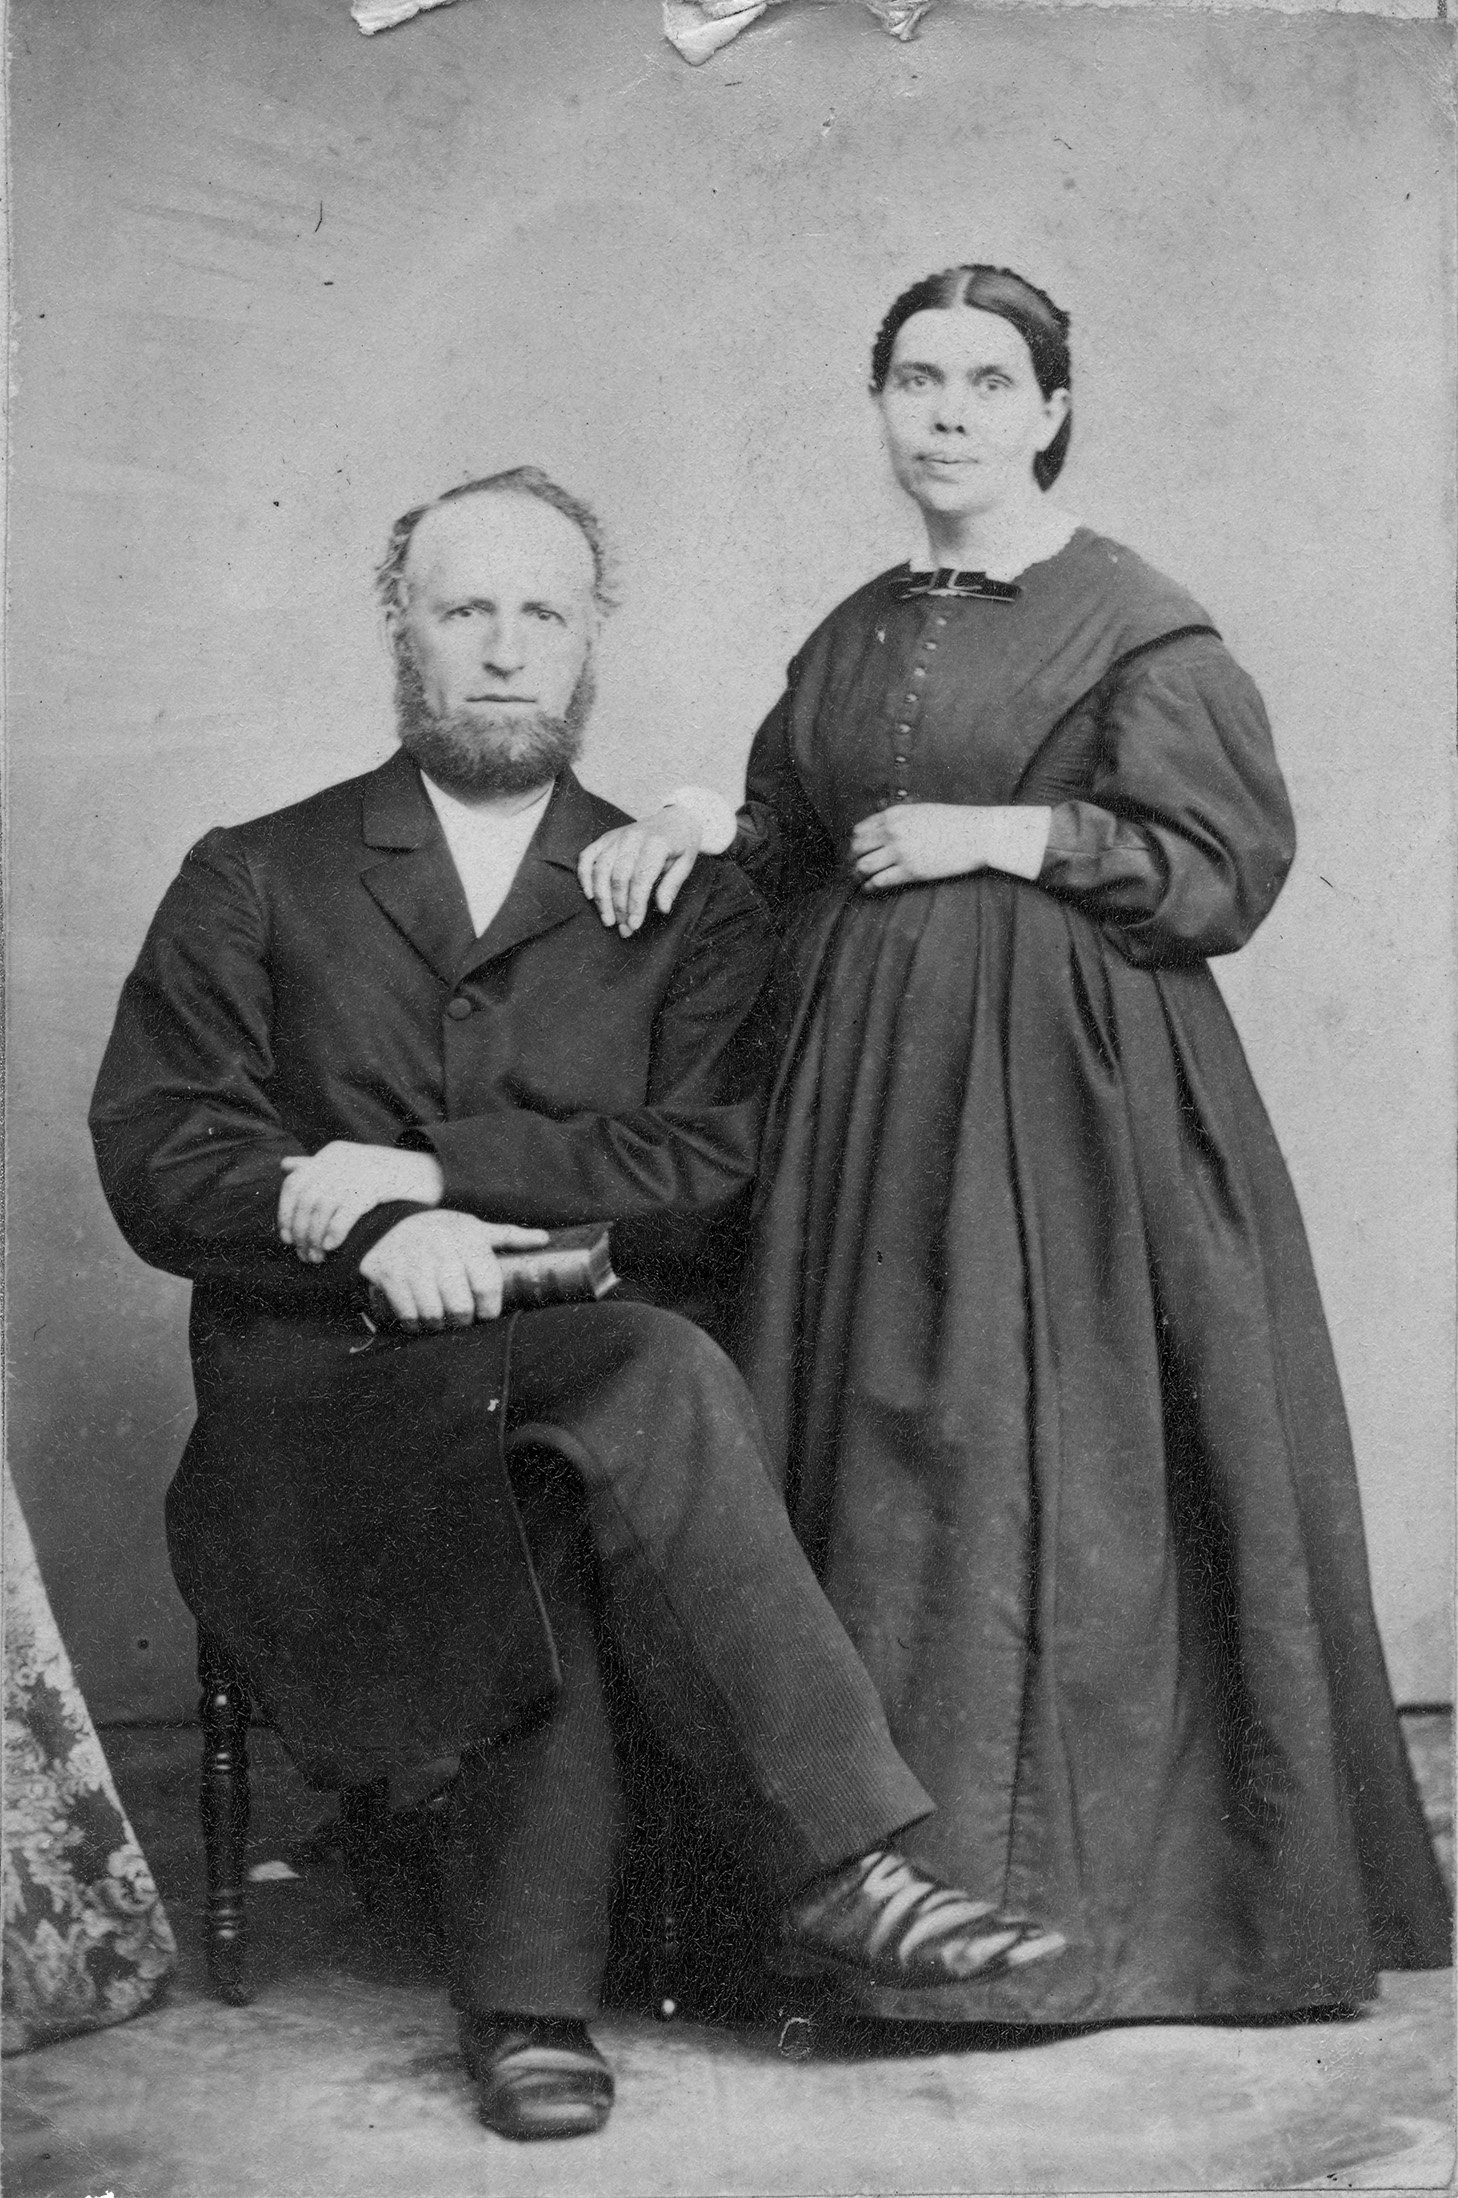
\includegraphics[width=1\linewidth]{images/james-and-ellen-white.jpg}
    \caption*{James Springer White (1821-1881) na Ellen White (1827-1915)}
    \label{fig:james-and-ellen-white}
\end{figure}

\othersQuote{\textbf{MWANADAMU aliumbwa kwa mfano wa Mungu}. ‘Mungu akasema, Na tumfanye mwanadamu kwa mfano wetu, baada ya namna yetu.’ ‘Basi Mungu akaumba mwanadamu kwa mfano wake, kwa mfano wa Mungu alimwumba.’ Mwanzo 1:26, 27. Ona pia sura ya. 9:6; 1 Wakorintho 11:7. \textbf{Wale wanaokataa Umbile la Mungu, wanasema kwamba ‘mfano’ hapa haimaanishi \underline{umbo la kimwili}, bali taswira ya kiadili, na wao hufanya hii iwe sehemu kuu ya kuanzia kuthibitisha kutokufa kwa watu wote}. Hoja inasimama hivi: Kwanza, mwanadamu aliumbwa kwa mfano wa Mungu wa kiadili. Pili, Mungu ni nafsi asiyeweza kufa. Tatu, kwa hiyo watu wote hawawezi kufa. Lakini namna hii ya kufikiri pia ingemthibitisha mwanadamu muweza wa yote, mjuzi wa yote, na aliye kila mahali, na hivyo kumvisha mwanadamu mwenye kufa sifa zote za mungu. Acheni tujaribu: Kwanza, mwanadamu aliumbwa kwa mfano wa Mungu wa kiadili. Pili, ni Mungu muweza wa yote, mjuzi wa yote, na aliye kila mahali. Tatu, kwa hivyo, mwanadamu ni muweza wa yote, mjuzi wa yote, na kila mahali. Kile ambacho kinathibitisha kupita kiasi, hakithibitishi chochote kwa uhakika, kwa hivyo msimamo kwamba mfano wa Mungu unamaanisha mfano wake wa maadili, hauwezi kudumu. \textbf{Kama ushahidi kwamba Mungu ni nafsi, soma maneno yake mwenyewe kwa Musa}: ‘Bwana akasema, Tazama, kuna mahali karibu nami, nawe utasimama juu ya mwamba; na itakuwa, wakati utukufu wangu ukipita, nitakuweka katika ufa wa mwamba, na kukufunika \textbf{kwa mkono wangu} \textbf{nikipita}. Nami nitauondoa \textbf{mkono wangu} nawe utaona \textbf{sehemu zangu za nyuma}; \textbf{lakini uso wangu haitaonekana}.’ Kutoka 33:21-23. Tazama pia sura. 24:9-11. \textbf{Hapa Mungu anamwambia Musa kwamba ataona \underline{umbo lake}}. \textbf{Kusema kwamba Mungu alimdhihirisha Musa kwamba aliona umbo lake, wakati yeye hana umbo, inamsingizia Mungu kwa kuongeza kwenye uwongo aina fulani ya mauzauza ya udanganyifu juu ya Musa mtumishi wake}.}[James S. White, PERGO 1.1; 1861][https://egwwritings.org/read?panels=p1471.3]

\othersQuoteNoGap{Lakini mwenye shaka anadhani anaona mgongano kati ya mstari wa 11, unaosema kwamba Bwana alizungumza na Musa uso kwa uso, na mstari wa 20, ambao unasema kwamba Musa hakuweza kuona uso wake. Wacha Hesabu 12:5-8 iondoe ugumu huo. \textbf{‘Na Bwana akashuka katika nguzo ya lile wingu}, akasimama mlangoni pa hema, akawaita Haruni na Miriamu, nao wote wawili wakatoka. Akasema, Sikieni sasa maneno yangu. Ikiwa kuna nabii kati yenu, mimi Bwana, nitajidhihirisha kwake katika maono, nami nitasema naye katika ndoto. Mtumishi wangu Musa si hivyo, ambaye ni mwaminifu katika nyumba yangu yote. \textbf{Pamoja naye nitazungumza mdomo kwa mdomo, hata \underline{kwa njia iliyo ya waziwazi}}.’}[James S. White, PERGO 2.1; 1861][https://egwwritings.org/read?panels=p1471.6]

\othersQuoteNoGap{Mungu mkuu na wa kutisha alishuka, akiwa amevikwa wingu la utukufu. \textbf{Wingu hili liliweza kuonekana, lakini si uso ambao una mng'ao zaidi kuliko elfu jua}. Chini ya hali hizi Musa aliruhusiwa kukaribia na \textbf{kuzungumza na Mungu uso kwa uso, au mdomo kwa mdomo, hata kwa njia iliyo ya waziwazi}.}[James S. White, PERGO 2.2; 1861][https://egwwritings.org/read?panels=p1471.7]

\othersQuoteNoGap{Nabii Danieli asema hivi, ‘Nikatazama hadi viti vya enzi vikashushwa, na \textbf{huyo mzee wa siku alikuwa ameketi}, ambaye vazi lake lilikuwa jeupe kama theluji, \textbf{na nywele za kichwa chake kama sufu safi}; \textbf{kiti chake cha enzi kilikuwa kama mwali wa moto, na magurudumu yake kama moto uwakao}.’ Sura 7:9. ‘Niliona katika maono ya usiku, na tazama, mmoja aliye kama Mwana wa Adamu akaja pamoja na mawingu ya mbinguni, na \textbf{akafika kwa huyo mzee wa siku}, wakamleta \textbf{karibu naye}, na pale akapewa uweza na utukufu na ufalme.’ Mistari ya 13, 14.}[James S. White, PERGO 2.3; 1861][https://egwwritings.org/read?panels=p1471.8]

\othersQuoteNoGap{Hapa kuna maelezo matukufu ya matendo ya \textbf{nafsi mbili}; yaani, \textbf{Mungu Baba, na Mwana wake Yesu Kristo}. \textbf{Kataa Umbile wao, na hakuna wazo tofauti katika nukuu hizi kutoka kwa Danieli}. Pamoja na nukuu hii soma tamko la mtume kwamba \textbf{Mwana alikuwa katika chapa dhahiri ya Umbile Wake}. ‘Mungu, ambaye nyakati za kale, na kwa njia nyingi alinena na baba zetu katika manabii, katika siku hizi za mwisho anasema nasi kupitia kwa Mwana, aliyemweka kuwa mrithi wa yote, tena kwa yeye aliumba ulimwengu; \textbf{ambaye ni mng'ao wa utukufu wake, na chapa dhahiri ya Umbile Wake}.’ Waebrania 1:1-3.}[James S. White, PERGO 3.1; 1861][https://egwwritings.org/read?panels=p1471.11]

\othersQuoteNoGap{Sisi hapa tunaongeza ushuhuda wa Kristo. ‘Na Baba mwenyewe aliyenituma alinishuhudia. Sauti yake hamjaisikia wakati wowote, \textbf{wala sura yake hamjaiona}.’ Yohana 5:37. Tazama pia Wafilipi 2:6. \textbf{Kusema kwamba Baba hana umbo la kibinafsi, inaonekana mkanganyiko ulio wazi zaidi wa maneno yaliyo wazi ya maandiko}. \\
PINGAMIZI. - ‘\textbf{\underline{Mungu ni Roho}}.’ Yohana 4:24.}[James S. White, PERGO 3.2; 1861][https://egwwritings.org/read?panels=p1471.12]

\othersQuoteNoGap{JIBU. - \textbf{Malaika pia ni roho} [Zaburi 104:4], lakini wale waliowatembelea Abramu na Lutu, Wakalala, wakala, wakaushika mkono wa Lutu. Walikuwa viumbe wa kiroho. \textbf{Vivyo hivyo Mungu ni Huluki wa kiroho}.}[James S. White, PERGO 3.3; 1861][https://egwwritings.org/read?panels=p1471.13]

\othersQuoteNoGap{OBJ. - \textbf{Mungu yuko kila mahali}. Ushahidi. Zaburi 139:1-8. \textbf{Yeye yuko zaidi katika kila mahali kama ilivyo katika sehemu nyingine}.}[James S. White, PERGO 3.4; 1861][https://egwwritings.org/read?panels=p1471.14]

\othersQuoteNoGap{ANS. - 1. \textbf{Mungu yuko kila mahali kwa uwezo wa kujua yote}, kama itakavyoonekana kwa maneno ya Daudi yaliyotajwa hapo juu. Mistari ya 1-6. ‘Ee Bwana, \textbf{umenichunguza, na kunijua mimi}. \textbf{Wewe wajua} kuketi kwangu na kuinuka kwangu; \textbf{unaelewa} mawazo yangu kwa mbali. Umeizunguka njia yangu na kulala kwangu, na \textbf{unazifahamu} njia zangu zote. Kwa maana hamna neno katika ulimi wangu, lakini, tazama, Ee Bwana, \textbf{wewe wajua kabisa}. Wewe umenizingira nyuma na mbele, ukaweka mkono wako juu yangu. \textbf{Ujuzi kama huo} ni wa ajabu sana kwangu. Uko juu; Siwezi kuufikia.’}[James S. White, PERGO 3.5; 1861][https://egwwritings.org/read?panels=p1471.15]

\othersQuoteNoGap{2. \textbf{Mungu yuko \underline{kila mahali kwa uwezo wa Roho wake}, \underline{ambaye ni mwakilishi wake}, na anadihirika popote apendapo}, kama itakavyoonekana kwa maneno ambayo mpingaji anadai, iliyotajwa hapo juu. Mistari wa 7-10. ‘\textbf{Niende wapi niiache \underline{Roho yako}}? \textbf{au nitakimbilia wapi kutoka kwa \underline{uwepo wako}}? Nikipanda mbinguni, wewe uko huko; nikitandika kitanda changu kuzimu, tazama, uko huko. Nikichukua mbawa za asubuhi, na kukaa pande za mwisho za bahari, hata huko mkono wako utaniongoza, na mkono wako wa kuume utanishika.’}[James S. White, PERGO 4.1; 1861][https://egwwritings.org/read?panels=p1471.18]

\othersQuoteNoGap{\textbf{Mungu yuko mbinguni}. Haya tunafundishwa katika maombi ya Bwana. ‘\textbf{Baba yetu uliye juu mbinguni}.’ Mathayo 6:9; Luka 11:2. \textbf{Lakini ikiwa Mungu yuko katika kila mahali kama alivyo mahali popote pamoja, basi mbingu pia iko katika kila mahali kama ilivyo mahali pamoja, na wazo la kwenda mbinguni yote ni makosa}. Sisi sote tuko mbinguni; na maombi ya Bwana, kulingana na teolojia hii ya ukungu ina maana kwa urahisi, Baba yetu \textbf{ambaye yuko kila mahali,} Jina lako litukuzwe. Ufalme wako na uje, mapenzi yako yatimizwe, duniani, \textbf{kama kila mahali}.}[James S. White, PERGO 4.2; 1861][https://egwwritings.org/read?panels=p1471.19]

\othersQuoteNoGap{Tena, wasomaji wa Biblia wameamini kwamba Enoko na Eliya kwa kweli walichukuliwa \textbf{hadi kwa Mungu mbinguni}. \textbf{Lakini ikiwa Mungu na mbingu ziko kila mahali kama ilivyo mahali pamoja, haya yote ni makosa}. Hawakutafsiriwa. Na yote yanayosemwa kuhusu gari la moto, na farasi wa moto, na upepo wa kisulisuli wa kumchukua Eliya juu mbinguni, ilikuwa tu gwaride ya upuzi. Walivukiza tu, na mvuke wa ukungu ukapita ulimwengu mzima. Hii ni yote kuhusu Enoko na Eliya ambayo akili inaweza kufahamu, \textbf{ikikubalika kwamba Mungu na mbingu wako katika sehemu moja kama vile kila mahali}. Lakini inasemwa juu ya Eliya kwamba ‘\textbf{alipanda} kwa kisulisuli \textbf{mbinguni}.’ 2 Wafalme 2:11. Na kuhusu Henoko inasemekana kwamba ‘alitembea pamoja na Mungu, naye hayuko, kwa kuwa Mungu alimchukua.’ Mwanzo 5:24.}[James S. White, PERGO 4.3; 1861][https://egwwritings.org/read?panels=p1471.20]

\othersQuoteNoGap{\textbf{Inasemekana Yesu yuko mkono wa kuume wa Ukuu huko juu}. Waebrania 1:3. ‘Basi, baada ya Bwana kusema nao \textbf{alichukuliwa \underline{juu mbinguni}}, \textbf{akaketi juu yake mkono wa kuume wa Mungu}.’ Marko 16:19. \textbf{Lakini ikiwa mbingu yuko kila mahali, na Mungu kila mahali, kisha kupaa kwa Kristo mbinguni, kwenye mkono wa kuume wa Baba, kunamaanisha tu kwamba yeye alienda kila mahali}! Alichukuliwa tu juu ambapo wingu lilimficha kutoka kwa macho ya wanafunzi wake, na kisha kuyeyuka na kwenda kila mahali! Ili kwamba badala ya Yesu mpendwa, iwe hivyo ilivyoelezwa kwa uzuri katika Agano zote mbili, tuna aina fulani tu ya kiini kilichotawanywa ulimwengu mzima. Na kupatana na theolojia hii iliyothibitishwa, ujio wa pili wa Kristo, au kurudi kwake itakuwa ni ufupisho wa kiini hiki kwa eneo fulani, sema mlima wa Mizeituni! \textbf{Kristo alifufuka kutoka kwa wafu akiwa na umbo la kimwili}. ‘Hayupo hapa,’ akasema malaika, ‘kwa maana  kafufuka kama alivyosema.’ Mathayo 28:6.}[James S. White, PERGO 5.1; 1861][https://egwwritings.org/read?panels=p1471.23]

\othersQuoteNoGap{‘Na walipokuwa wakienda kuwaambia wanafunzi wa Yesu tazama, Yesu akakutana nao, akiwasalimu, Salamu! Na wao wakaja \textbf{wakamshika miguu}, wakamsujudia.’ Mstari wa 9.}[James S. White, PERGO 5.2; 1861][https://egwwritings.org/read?panels=p1471.24]

\othersQuoteNoGap{‘\textbf{Tazama mikono yangu na miguu yangu},’ Yesu akawaambia wale waliokuwa na shaka kuhusu ufufuo wake, ‘kwamba ni mimi mwenyewe. \textbf{Nishikeni mwone, \underline{maana roho haina nyama na mifupa} kama mnavyoniona ninavyo}. Naye akiisha kusema hayo, \textbf{akawaonyesha mikono yake na miguu yake}. Na walipokuwa bado hawajaamini kwa furaha, wakistaajabu, akawaambia, Je! mna nyama yoyote? Wakampa kipande cha samaki wa kuokwa, na sega la asali, akakitwaa na kula mbele yao.’ Luka 24:39-43.}[James S. White, PERGO 5.3; 1861][https://egwwritings.org/read?panels=p1471.25]

\othersQuoteNoGap{Baada ya Yesu kusema na wanafunzi wake katika mlima wa Mizeituni, \textbf{alipandishwa kutoka kwao}, na wingu likampokea kutoka machoni pao. ‘Na huku wakitazama kwa uthabiti \textbf{alipokuwa akienda mbinguni,} tazama, watu wawili wakasimama karibu nao, wenye mavazi meupe, wakasema, Ninyi Enyi watu wa Galilaya, mbona mmesimama mkitazama mbinguni? Yesu huyu huyu ambaye \textbf{amechukuliwa juu kutoka kwenu kwenda mbinguni}, atakuja jinsi iyo hiyo mlivyomwona \textbf{akienda zake mbinguni}.’ Matendo 1:9-11. J. W.}[James S. White, PERGO 6.1; 1861][https://egwwritings.org/read?panels=p1471.27]

James White fights the idea that God is just a spirit, and as such, is present \others{as much in every place as in any one place}. He gives plain and positive testimony from Scripture that God is a personal being; we see the very same sentiments in Ellen White’s writings.

James White anapinga wazo la kwamba Mungu ni roho tu, na kwa hivyo, yuko \others{zaidi kila mahali kama mahali pamoja}. Anatoa ushuhuda wa wazi na chanya kutoka katika Maandiko kwamba Mungu ni huluki binafsi; tunaona hisia sawa katika maandishi ya Ellen White.

\egw{Nguvu kuu inayofanya kazi kupitia maumbile yote na kutegemeza vitu vyote si, kama watu wengine wanasayansi wanavyodai, \textbf{kanuni inayoenea tu}, nishati inayofanya kazi. \textbf{\underline{Mungu ni roho; lakini Yeye ni huluki binafsi}}, \textbf{kwa maana mwanadamu aliumbwa kwa mfano Wake}. \textbf{Kama \underline{mtu binafsi}}, Mungu amejidhihirisha katika Mwanawe. Yesu, mng'ao wa utukufu wa Baba, “na \textbf{mfano halisi \underline{wa nafsi yake}}” (Waebrania 1:3), alikuwa duniani alionekana katika umbo kama mwanadamu. Kama \textbf{Mwokozi binafsi} Alikuja ulimwenguni. Kama \textbf{Mwokozi binafsi alipaa \underline{juu}}. Kama \textbf{Mwokozi wa kibinafsi Yeye hufanya maombezi \underline{katika nyua za mbinguni}}. \textbf{Mbele ya kiti cha enzi cha Mungu} kwa niaba yetu wanadamu “Mmoja kama Mwana wa binadamu.” Danieli 7:13.}[Ed 131.5; 1903][https://egwwritings.org/read?panels=p29.632]

Ellen White na waanzilishi wa Waadventista walifanya tofauti kati ya maneno ‘roho’ na ‘huluki’. Mungu ni huluki binafsi, si roho tu. Yeye hayuko\others{zaidi katika kila mahali kama mahali pamoja}, lakini Yeye yuko\others{mahali pamoja zaidi ya mahali pengine}[John. N. Loughborough, “Is God a Person?” The Adventist Review and Sabbath Herald, September 18, 1855][https://documents.adventistarchives.org/Periodicals/RH/RH18550918-V07-06.pdf]. Yuko mbinguni, katika hekalu lake, ameketi juu ya kiti Chake cha enzi—katika nafsi yake—na Yeye yuko kila mahali kupitia kwa mwakilishi Wake, Roho mtakatifu.

Hapa kuna manukuu mengine kutoka kwa Dada White ambayo yanapatana na waanzilishi katika maoni juu ya \emcap{ubinafsi wa Mungu}:

\egw{Yeye \normaltext{[Yesu]} alifundisha kwamba Mungu ni mthawabishaji wa wenye haki, na muadhibu wa wenye kuvunja sheria. \textbf{Hakuwa roho isiyoshikika}, bali mtawala aliye hai wa ulimwengu. \textbf{Huyu Baba mwenye neema} alikuwa akifanya kazi kila mara kwa ajili ya wema wa mwanadamu, na kukumbuka yote hayo inayomhusu...}[3SP 47.1; 1878][https://egwwritings.org/read?panels=p142.195]

\egw{\textbf{Biblia inatuonyesha \underline{Mungu katika mahali pake pa juu na patakatifu}}, si katika hali ya kutotenda, si katika ukimya na upweke, lakini amezungukwa na elfu kumi mara elfu kumi na maelfu ya maelfu ya viumbe watakatifu, wote wakingoja kufanya mapenzi Yake. \textbf{Kupitia wajumbe hawa Yeye yuko katika mawasiliano hai na kila sehemu ya utawala Wake}. \textbf{\underline{Kupitia kwa Roho wake yuko kila mahali}}. \textbf{Kupitia wakala wa Roho wake na malaika zake} anawahudumia watoto wa wanaume.}[MH 417.2; 1905][https://egwwritings.org/read?panels=p135.2136]

\egw{Ukuu wa Mungu kwetu sisi haueleweki. ‘\textbf{Kiti cha enzi cha Bwana ki mbinguni}’ (Zaburi 11:4); \textbf{\underline{lakini kwa Roho wake yuko kila mahali}}. \textbf{Ana ujuzi wa ndani} wa, na shauku ya kibinafsi katika, kazi zote za mkono Wake.}[Ed 132.2; 1903][https://egwwritings.org/read?panels=p29.636]

\egw{Kupitia Yesu Kristo, \textbf{Mungu—si manukato, \underline{si kitu kisichoshikika}, \underline{bali Mungu binafsi}}—aliyemuumba mwanadamu na kumpa akili na uwezo.}[Ms117-1898.10; 1898][https://egwwritings.org/read?panels=p7182.15]

Tukiendelea katika kijitabu cha James White, tunasoma ukosoaji wake mkali juu ya dhana ya Mungu asiye na mwili. Kabla ya hapo, hebu tukumbuke kwa ufupi hoja ya Dk. Kellogg kwamba\others{\textbf{\underline{Majadiliano kuhusu umbo la Mungu hayana faida kabisa}}}[Dr. John H. Kellogg, The Living Temple, p.33.][https://archive.org/details/J.H.Kellogg.TheLivingTemple1903/page/n33/] kwa sababu Mungu \others{\textbf{yuko mbali sana na sisi \textbf{\underline{kwa ufahamu kama vile ilivyo mipaka ya nafasi na wakati}}}}. Aliamini kwamba nafsi ya Mungu haizuiliwi katika eneo moja kwa sababu Yeye yuko\others{zaidi kila mahali kama mahali pamoja}[James S. White, PERGO 4.3; 1861][https://egwwritings.org/read?panels=p1471.20] \footnote{Katika Hekalu Hai, Dk. Kellogg alipinga kwamba Mungu hawezi kuwa kila mahali kwa wakati mmoja: “\textit{Asema mmoja}, ‘Mungu anaweza kuwepo kwa Roho wake, au kwa nguvu zake, lakini hakika Mungu mwenyewe \textit{hawezi kuwepo kila mahali kwa wakati mmoja}.’ Tunajibu: Nguvu zinawezaje kutenganishwa na chanzo cha nguvu? Mahali ambapo Roho wa Mungu anafanya kazi, mahali ambapo nguvu za Mungu zinadhihirishwa, Mungu \textit{mwenyewe kwa kweli na kwa hakika yupo}…“ \href{https://archive.org/details/J.H.Kellogg.TheLivingTemple1903/page/n29/}{John H. Kellogg, The Living Temple, p.28}.}. Ikiwa Mungu katika ubinafsi Wake angekuwa huluki dhahiri, mwenye mwili unaoshikika, basi hangeweza kuwepo\others{zaidi kila mahali kama mahali pamoja} na, hivyo, kudumisha maisha. James White anaendelea dhidi ya hoja kwamba Mungu hana mwili katika nafsi yake.

\othersQuote{KUTOKUWA NA MWILI}

\othersQuoteNoGap{\textbf{HILI ni jina lingine tu la chaupepeta}. \textbf{Ni hasi ya vitu} \textbf{vyote na} \textbf{\underline{huluki} }- ya vyote kuwepo. Hakuna chembe hata moja cha uthibitisho wa kuendelezwa ili kuthibitisha kuwepo kwake. Haina njia ya kujidhihirisha kwa akili yoyote mbinguni au nchini. \textbf{Mungu, malaika, na wanadamu hawawezi kufikiria kitu kama hicho, kiumbe au kitu kama hicho}. \textbf{Haimiliki mali au nguvu yoyote ambayo kwayo \underline{inaweza kujidhihirisha kwa kiumbe chochote chenye akili ulimwenguni}}. Wazo na mlinganisho kamwe haziichanganui, au hata kuziifikiria. \textbf{Ufunuo kamwe haufichui wala hakuna hisia zetu kushuhudia kuwepo kwake}. \textbf{Haiwezi kuonekana, kuhisika, kusikika, kuonjeka, au kunusika, hata kwa viungo vya nguvu zaidi, au hisia kali zaidi}. Sio kioevu au ngumu, laini au ngumu - haiwezi kupanua au kupungua. Kwa ufupi, haiwezi kuwa na ushawishi wowote - haiwezi kuchukua hatua au kutekelezwa. Na hata kama ipo, haiwezi kutumika. Haina mtu yeyote, mali inayohitajika, kitivo, au kazi, hata hivyo, ajabu kusema, \textbf{kutokuwa na mwili ni Mungu wa Mkristo wa kisasa}, \textbf{mbingu yake anayotarajia}, \textbf{nafsi yake isiyoweza kufa} - \textbf{yake yote}!}[James S. White, PERGO 6.2; 1861][https://egwwritings.org/read?panels=p1471.29]

\othersQuoteNoGap{\textbf{Enyi madhehebu! O Asiyeamini Mungu!! O maangamizi!!!} \textbf{nani anaweza kutambua vivuli vyema vya tofauti kati ya moja na nyingine?} Wanaonekana sawa, wote isipokuwa kwa jina. \textbf{Mkana Mungu hana Mungu. \underline{Mdhehebu ana Mungu asiye na mwili au sehemu}.} Nani anaweza kufafanua tofauti? Kwa upande wetu hatuoni tofauti ya unywele mmoja; \textbf{wote wawili wanadai kuwa hasi ya vitu vyote vilivyopo} - na vyote viwili havina nguvu na havijulikani.}[James S. White, PERGO 6.3; 1861][https://egwwritings.org/read?panels=p1471.30]

\othersQuoteNoGap{\textbf{Mtu asiyeamini kuwa kuna Mungu hana maisha ya baadaye, zaidi ya kaburi. Mdhehebu ana moja, \underline{lakini haionekani, kama Mungu wake; na bila mwili au sehemu}. Hapa tena wote wawili ni hasi, na wote wawili wanafika katika hatua moja}. Imani na tumaini lao ni sawa; ila inaonyeshwa kwa maneno tofauti.}[James S. White, PERGO 7.1; 1861][https://egwwritings.org/read?panels=p1471.33]

\othersQuoteNoGap{Tena, \textbf{asiyeamini Mungu hana mbingu katika umilele}. \textbf{Mdhehebu ana mmoja, lakini \underline{haionekani katika mali zake zote}, na kwa hiyo hasi katika mali na vitu vyote}. Hapa tena wako sawa, na wanafikia hatua sawa.}[James S. White, PERGO 7.2; 1861][https://egwwritings.org/read?panels=p1471.34]

\othersQuoteNoGap{Kwa kuwa hatuwaonei wivu kumiliki yote wanayodai, sasa tutawaacha kwa starehe na utulivu bila wasiwasi yoyote na kuendelea kuchunguza sehemu ambayo bado imesalia ili wanaopenda mali waliodharauliwa wafurahie.}[James S. White, PERGO 7.3; 1861][https://egwwritings.org/read?panels=p1471.35]

\othersQuoteNoGap{\textbf{Mungu ni nini? Yeye ni dutu, akili iliyopangwa, \underline{anamiliki mwili na sehemu}. Mwanadamu ni mfano wake.}}[James S. White, PERGO 7.4; 1861][https://egwwritings.org/read?panels=p1471.36]

\othersQuoteNoGap{\textbf{Yesu Kristo ni nini? Yeye ni Mwana wa Mungu, na ni \underline{kama Baba yake}, akiwa ‘mng'ao wa utukufu wa Baba yake, na mfano halisi wa nafsi yake.’ \underline{Yeye ni dutu, mwenye akili, mwili, sehemu} na hamu; mwenye mwili usiokufa na mifupa isiyoweza kufa}.}[James S. White, PERGO 7.5; 1861][https://egwwritings.org/read?panels=p1471.37]

\othersQuoteNoGap{\textbf{Wanadamu ni nini?} Hao ni watoto wa Adamu. \textbf{Wana uwezo wa kupokea akili na kuinuliwa kwa kiwango cha \underline{kufufuliwa kutoka kwa wafu na kuwa na mwili kama ule wa Yesu Kristo}, \underline{na kuwa na mwili na mifupa isiyoweza kufa}}. Wakikamilishwa hivyo, watamiliki \textbf{ulimwengu unaoonekana}, yaani, dunia, kuwa ‘urithi wao wa milele.’ Tukiwa na matumaini na matarajio haya mbele yetu, tunasema kwa ulimwengu wa Kikristo unaoshikilia kutoonekana, kwamba wanakaribishwa kwa Mungu wao - maisha yao - mbinguni yao, na yote yao. Wanadai yale tunayoyatupa; na hatudai ila hayo wanayoyatupa. \textbf{Kwa hiyo, hakuna sababu ya ugomvi au ugomvi kati yetu}.}[James S. White, PERGO 7.6; 1861][https://egwwritings.org/read?panels=p1471.38]

\othersQuoteNoGap{Tunachagua vitu vyote vinavyoshikika – vilivyobaki \\
Madhehebu wa kimafumbo anapata; \\
Kila anachodai kila mmoja anacho, \\
Wala usichukie furaha ya kila mmoja. \\
Mungu asiye na mwili wanamchagua, \\
Kwa Mungu wa namna hii hatuna faida; \\
\textbf{Mbingu na kuzimu isiyoonekana,} \\
\textbf{Katika mbingu kama hii hatuwezi kukaa.} \\
\textbf{Tunadai ardhi, hewa na anga,} \\
\textbf{Na ulimwengu wote wa nyota huko juu;} \\
\textbf{Dhahabu, fedha, madini na vito vya thamani,} \\
\textbf{Na miili iliyotengenezwa kwa nyama na mifupa.} \\
\textbf{Hili ndilo tumaini letu, mbingu yetu, yetu yote,} \\
\textbf{Tunapokombolewa mara moja kutoka katika anguko la Adamu;} \\
\textbf{Vitu vyote ni vyetu, nasi tutakuwa,} \\
\textbf{Wa Bwana milele zote}.}[James S. White, PERGO 8.1; 1861][https://egwwritings.org/read?panels=p1471.41]

James White alilinganisha Maoni juu ya Mungu asiyeonekana na matengano, Makufuru, na maangamizi. “Mungu Asiye na mwili” ni usemi mwingine sawia na kutokuwepo kwa Mungu. James White hakuwahi kupokea karipio lolote kutoka kwa Dada White kwa maoni haya; badala yake, yaliungwa mkono na maandishi yake. Wengi wanadai kwamba Dada White alibadilisha maoni yake baada ya muda na, baadaye, alikubali fundisho la Utatu, lakini hilo haliungwi mkono na rekodi za kihistoria zenye kina. Mnamo 1905, Dada White anakumbuka tukio na Dk. Kellogg wakati, miaka ishirini nyuma, alikuja kwake na hisia zilezile kuhusu Umbile la Mungu ambazo James White na waanzilishi wengine walikuwa wanakanusha:

\egw{Sasa somo hili limehifadhiwa mbele yangu kwa zaidi ya miaka ishirini. Mume wangu amekufa miaka ishirini, na kabla hajafa, mambo yaliingia. Dk. Kellogg aliingia chumbani kwangu; Nilikuwa nimechukua mojawapo wa chumba kikubwa cha ofisi kama nyumba yangu. Nilikuwa na vyumba viwili au vitatu huko, na \textbf{akapata nuru kuu}; akaketi, na kusema nuru yake hiyo: \textbf{ilikuwa nadharia au makosa sawa na elimu ya kisasa ambayo anawasilisha, na aliliwasilisha katika ‘Living Temple.’} Nikamwambia, ‘Dakt. Kellogg, \textbf{nimekutana na hayo.}’ Nilikutana nayo nilipoanza kusafiri. Nilikutana nayo Kaskazini; Nilikutana nayo huko New Hampshire. Niliona laana ya ushawishi wake huko Massachusetts, na \textbf{shuhuda nilizopewa ziligonga hadi hatukukwa na chochote cha namna hiyo kufunzwa katika makanisa yetu}. Na nikazungumza pamoja naye. \textbf{Nikampa historia}--sina wakati wa kukupa hapa. \textbf{Nikampa historia jinsi hilo lilishughulikiwa na Roho wa Mungu, na jinsi sisi kama watu tunafaa tuepuke ujanja na udanganyifu}. Na ni watumishi waliokuwa wakiwahadaa watu kwa elimu hizi za kisasa. \textbf{Sitakuelezea walichokiendeleza}--\textbf{huenda kinawezastahili kuja}; lakini sitakuambia sasa walichoendeleza; \textbf{lakini nitakuambia nini elimu hii ya kisasa inaongoza kwayo:} \textbf{Inaongoza kwa \underline{kwa kutokuwepo wa Kristo, kwa kutokuwepo wa Mungu}, \underline{ubinafsi wake}, na kuleta ndani,—nikiite nini?—aina ya \underline{nadharia iliyobuniwa ya Mungu na Kristo}}.}[Ms70a-1905.11; 1905][https://egwwritings.org/read?panels=p12696.17]

Maoni ya Kellogg katika Hekalu Hai kuhusu \emcap{ubinafsi wa Mungu} yanaongoza kwa kutokuwepo kwa utu uzima wa Kristo na vilevile utu uzima wa Mungu. Kwa nini? Kwa sababu maoni yake juu ya Mungu yanadai Mungu asiye na mwili. Kanisa lilikabiliwa na hisia kama hizo mwanzoni mwa kazi yao. James White aliandika kuwahusu katika kijitabu chake “\textit{Ubinafsi wa Mungu}”, na Dada White alikumbuka uzoefu wao wa mapema wakati yeye na mume wake walipambana na kosa la kwamba Mungu ni roho isiyoonekana, inayotawala yote.

% The personality of God by James White
% This article already has a poem, so there is no need for another one

% The personality of God by James White
% This article already has a poem, so there is no need for another one
